\chapter{Model i Druk 3D}
\begin{figure}[h!]
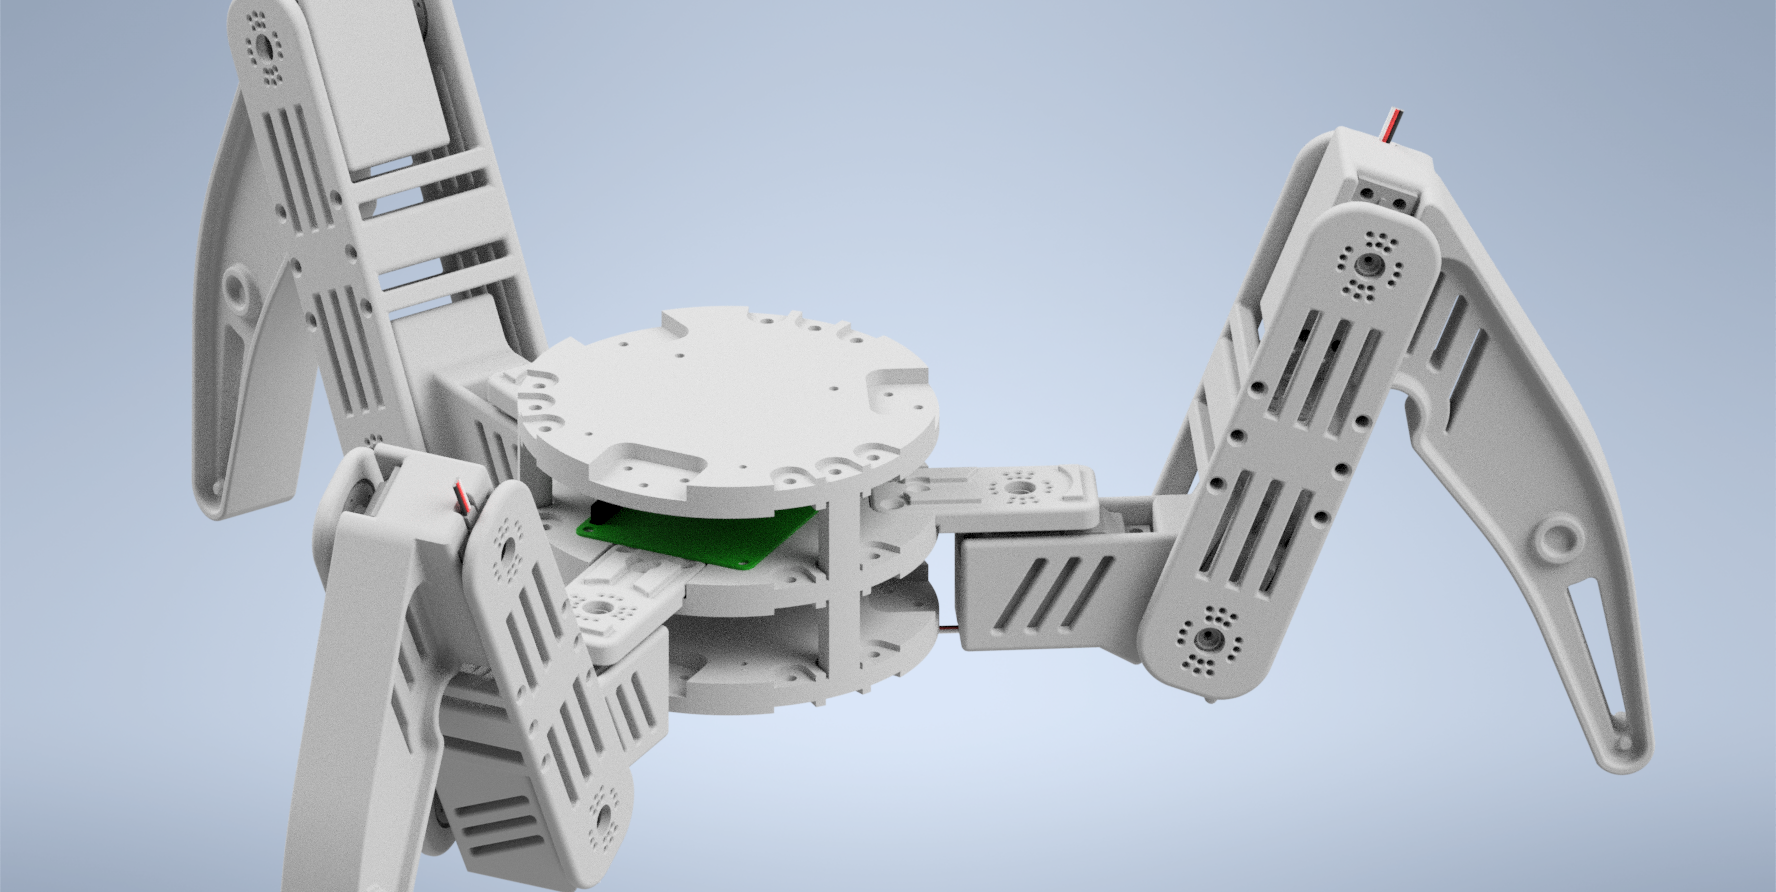
\includegraphics[width=\textwidth]{img/CAD_assembly.png}
\caption{Model złożeniowy.}
\label{CAD_assembly}
\end{figure}
Jedym z głównych założeń projektu była możliwość wydrukowania całej konstrukcji w 3D. Miało to na celu znaczne obniżenie kosztów produkcji, ale przede wszystkim umożliwić znacznie szybsze przeróbki. Jest to o tyle istotne, że prowadzone będą badania z algorytami chodu - w przypdaku większości algorytmów wydłużenie pewnych elementów nogi może zmniejszyć wymagane prędkości ruchu serw. Eksperymenty takie mogą wymusić liczne przedruki poszczególnych członów nóg robota.\\

Drugim założeniem projektowym stojącym za konstrukcją taką jak na rysunku \ref{CAD_assembly} jest modularność. Bardzo podobną modularność oferuje robot TurtleBot 3, który także był inspiracją stojącą za konstrukcją. Turtlebot składa się z wielu identycznych warstw, które zawierają liczne otwory montażowe umożliwiające przykręcenie w zasadzie dowolnego elemnentu. Projekt robiony w ramach tej pracy został oparty o podobną ideę. Także składa się z wielu identycznych warstw zawierających liczne otwory montażowe. Otwory te zostały dobrane pod kątem elektroniki jaka będzie montowana, ale na każdej z warstw można zamontować dowolny element w jednej z kilku konfiguracji.\\

Zostały także dokładnie zwymiarowane otwory montażowe znajdujące się na orczykach do zakupionych serw i przeniesione na poszczególne elementy nóg. Do montażu wspomnianych orczyków zakupione zostały śruby $M1.6$, co stanowi swojego rodzaju drobny eksperyment. Zwykle orczyki montuje się za pomocą kleju lub wkrętów dostarczanych wraz z serwomechanizmem. Są to jednak metody przynajmniej częściowo destrukcyjne - nie umożliwiają szybkiego demontażu i wymiany elementów, co jest bardzo ważnym elementem tego projektu. Zastosowanie śrub z nakrętkami rozwiązuje ten problem - jednak pojawia się pytanie czy nie generuje to innych problemów. Bardzo prawdopodobne jest pojawienie się problemu z samoodkręcającymi się śrubkami przy dłuższym użytkowaniu - zjawisko spowodowane drganiami generowanymi przez serwa. Było to już problemem w przypadku innych projektów - gdzie serwa odkręcały się od orczyków. Jednakże projekty tamte wykonane były w technologii CNC z blachy lub włókna węglowego - nigdy nie były drukowane w 3D. Bardzo możliwe jest że filament wytłumi drgania.

Oryginalny projekt zawiera także pewną wadę konstrukcyjną - jest to bardzo cienki element łączący nogę z tułowiem (element nogi zero). Istnieje duże ryzyko gięcia a może nawet łamania się wyżej wymienionego elementu. Aby zmniejszyć to ryzyko, wspomniany element został miejscami pogrubiony i zakupione zostały (TODO - trzeba kupić) metalowe orczyki. Najtrwalszym rozwiązaniem oczywiście byłoby stowrzenie dodatkowego elementu który byłby przytwierdzony do dolnej części obudowy i posiadałby oś obrotu z pierwszym elementem nogi -  "podtrzymywałby" ten elemnt od dołu.\\

Całość konstrukcji została zaprojektowana w programie Autodesk Inventor. Program ten został wybrany tylko i wyłącznie ze względu na fakt, że był autorowi projektu dość dobrze znany.\\

Modele zostały wydrukowane na drukarce Zortrax M200. Została ona wybrana ze względu na jej dostępnośc na uczelni. Dodatkowo, aby przygotować pliki pod druk, należało model przetworzyć programem Z-Suite. W programie większość ustawień pozostawiana była bez zmian, jedynie 2 istotne ustawienia zostały dostosowane do projektu. Zostało ustawione minimalne niezerowe wypełnienie, około $10\%$ i warstwy, wierzchnia i spodnia, zostały ustawione na najgrubsą możliwą opcję. Ustawienia te znalezione zostały eksperymentalnie - wydają się najlepiej balansować między wytrzymałością a czasem druku i ilością zużytego materiału. Dodatkowo, przed ostatecznym wydrukiem, wewnątrz programu inventor, zwiększone zostały o około $0.3-0.4 mm$ wszystkie otwory montażowe, ponieważ modele "puchną" i dziury te po wydruku były znacznie mniejsze niż na tworzonych szkicach.\\
